\documentclass[11pt, twoside]{article}

\usepackage{graphicx}
\usepackage{amsmath}
\usepackage{amssymb}
\usepackage{verbatim} 
\usepackage{subfigure}
\usepackage{amsfonts}
\usepackage{hyperref}
%\usepackage{tikz}



\RequirePackage[usenames,dvipsnames]{color}
\RequirePackage{fancyhdr}
\RequirePackage{graphicx}

% to include C++ code:
\usepackage{listings}
\usepackage{xcolor}
\lstset { %
	language=C++,
	backgroundcolor=\color{black!5}, % set backgroundcolor
	basicstyle=\footnotesize,% basic font setting
}

%------------------- settings margini ----
\setlength{\oddsidemargin}{-15pt}
\setlength{\evensidemargin}{-15pt}
\setlength{\marginparwidth}{0pt}
\setlength{\textwidth}{500pt}
\setlength{\topmargin}{-40pt}
\setlength{\textheight}{650pt}

\newcommand{\cambiaFont}[2]{{\fontencoding{T1}\fontfamily{#1}%
		\selectfont#2}}

%-------- pacchetti base------------------
\usepackage[english]{babel}
\usepackage{euscript}
\usepackage[utf8]{inputenc}
%------ per i diagrammi commutativi: 
\usepackage{pictexwd,dcpic}
\usepackage[all]{xy}

%---- fancyheader and footer 
%\fancyhead{} % clear all fields
%\fancyhead[LE]{\thepage~~~~\textrm{asdf}~~\textit{asdffda}}
%\fancyhead[RO]{ {\sf Ricerca di Crittografia}, ~~~~\thepage}
\fancyfoot{}
\fancyfoot[RO]{ {\small  MPHYG002: Research Computing with C++, ~\thepage}}
\fancyfoot[LE]{ {\small \thepage,~ Coursework 2 }}
\renewcommand{\headrulewidth}{0.0pt}



\begin{document}

% %--------- pagenumbering ------------
\setcounter{page}{1}
\pagestyle{fancy} 
% %----------------------------------------



% ----  TITLE DATE ---- 
~\vspace{-2cm} 
\begin{center}  	
	
	\hrule
	
	\vspace{0.5cm} 
	\color{Black} MPHYG002: Research Computing with C++ \color{Black}
	\vspace{0.5cm} \\
	\cambiaFont{ppl}{ \color{MidnightBlue} $\bullet$ \color{MidnightBlue} ~{\Large Coursework 2 - Conway's Game of Life } ~ \color{MidnightBlue}$\bullet$\color{black}} 
	\vspace{0.3cm} \\
	Sebastiano Ferraris  ~ SN: 14108168 ~  s.ferraris@ucl.ac.uk ~ \today 
	\vspace{0.5cm} 
	\hrule
	
\end{center}

\vspace{0.1in}


%--- autore



%------------ indice eventuale:
 %\tableofcontents
%____________________________


\begin{center}
	\color{MidnightBlue} {\Large Introducing the Game }\color{Black} 
\end{center}

\noindent
\href{https://en.wikipedia.org/wiki/Conway%27s_Game_of_Life}{Conway's Game of Life} is a deterministic evolutionary discrete event dynamical system played on an infinite 2-dimensional grid.
At each position of the gird there is a cell, that can be in two states: \emph{alive} 1, or \emph{dead} 0.
The state of cell $C$ at time $t$, indicated with $\text{state}_t(C)$ evolves over a discrete time according to its degree. The degree of a cell, $\text{deg}_t(C)$ is the number of alive cells into its eight neigbours, and the evolution model from the state $t$ to the state $t+1$ happens according to the following rules, called update rule, applied simultaneously for all the cells in the grid for a given time-state:
\begin{enumerate}
	\item $\text{state}_t(C) = 1$ and $\text{deg}_t(C)<2$ then $\text{state}_{t+1}(C) = 0$.
	\item $\text{state}_t(C) = 1$ and $2 \leq\text{deg}_t(C) \leq 3$ then $\text{state}_{t+1}(C) = 1$.
	\item $\text{state}_t(C) = 1$ and $\text{deg}_t(C)>3$ then $\text{state}_{t+1}(C) = 0$.
	\item $\text{state}_t(C) = 0$ and $\text{deg}_t(C)=3$ then $\text{state}_{t+1}(C) = 1$.
\end{enumerate}
The initial state is called \emph{seed}, and it completely determines the subsequent steps of the game.

\begin{center}
	\color{MidnightBlue} {\Large Part 1: Serial Solution }\color{Black} 
\end{center}

\noindent
In the simple implementation here proposed, a \emph{state} is represented by a \emph{.txt} file that contains a binary matrix whose zeros represents the dead cells and ones represents the living cells. A \emph{game}, in the perspective here proposed, is a sequence of $.txt$ file where in the filename appears the name of the game, shared for each state, and an integer time parameter, starting from $0$ for the seed. Two states with consecutive indexes are related to each others by the update rule.
Given the need of plotting computing statistics for computational comparisons purposes and of obtaining an animation of a game (see the README.md on github \href{https://github.com/SebastianoF/game_of_life}{repository}), I opted for wrapping the C++ code inside python with boost::python, and to call the shared object (.so) generated with the C++ compiler as libraries inside python code. \\

\noindent
\color{MidnightBlue} {\Large Design and code structure }\color{Black}  \\
The object oriented structure is driven by the definition of state and game. To reduce computational costs and the length of the code, there is no class implemented for a state or a game, being structured .txt files. The classes are implemented for the operations between states, as well as to create random seeds, visualize state and games.

The object oriented structure for the Python code is given by the following classes:


While the C++ code, called as a library in the python code, has the structure:


Folders:


%\begin{figure}[htbp]
%	\centering
%	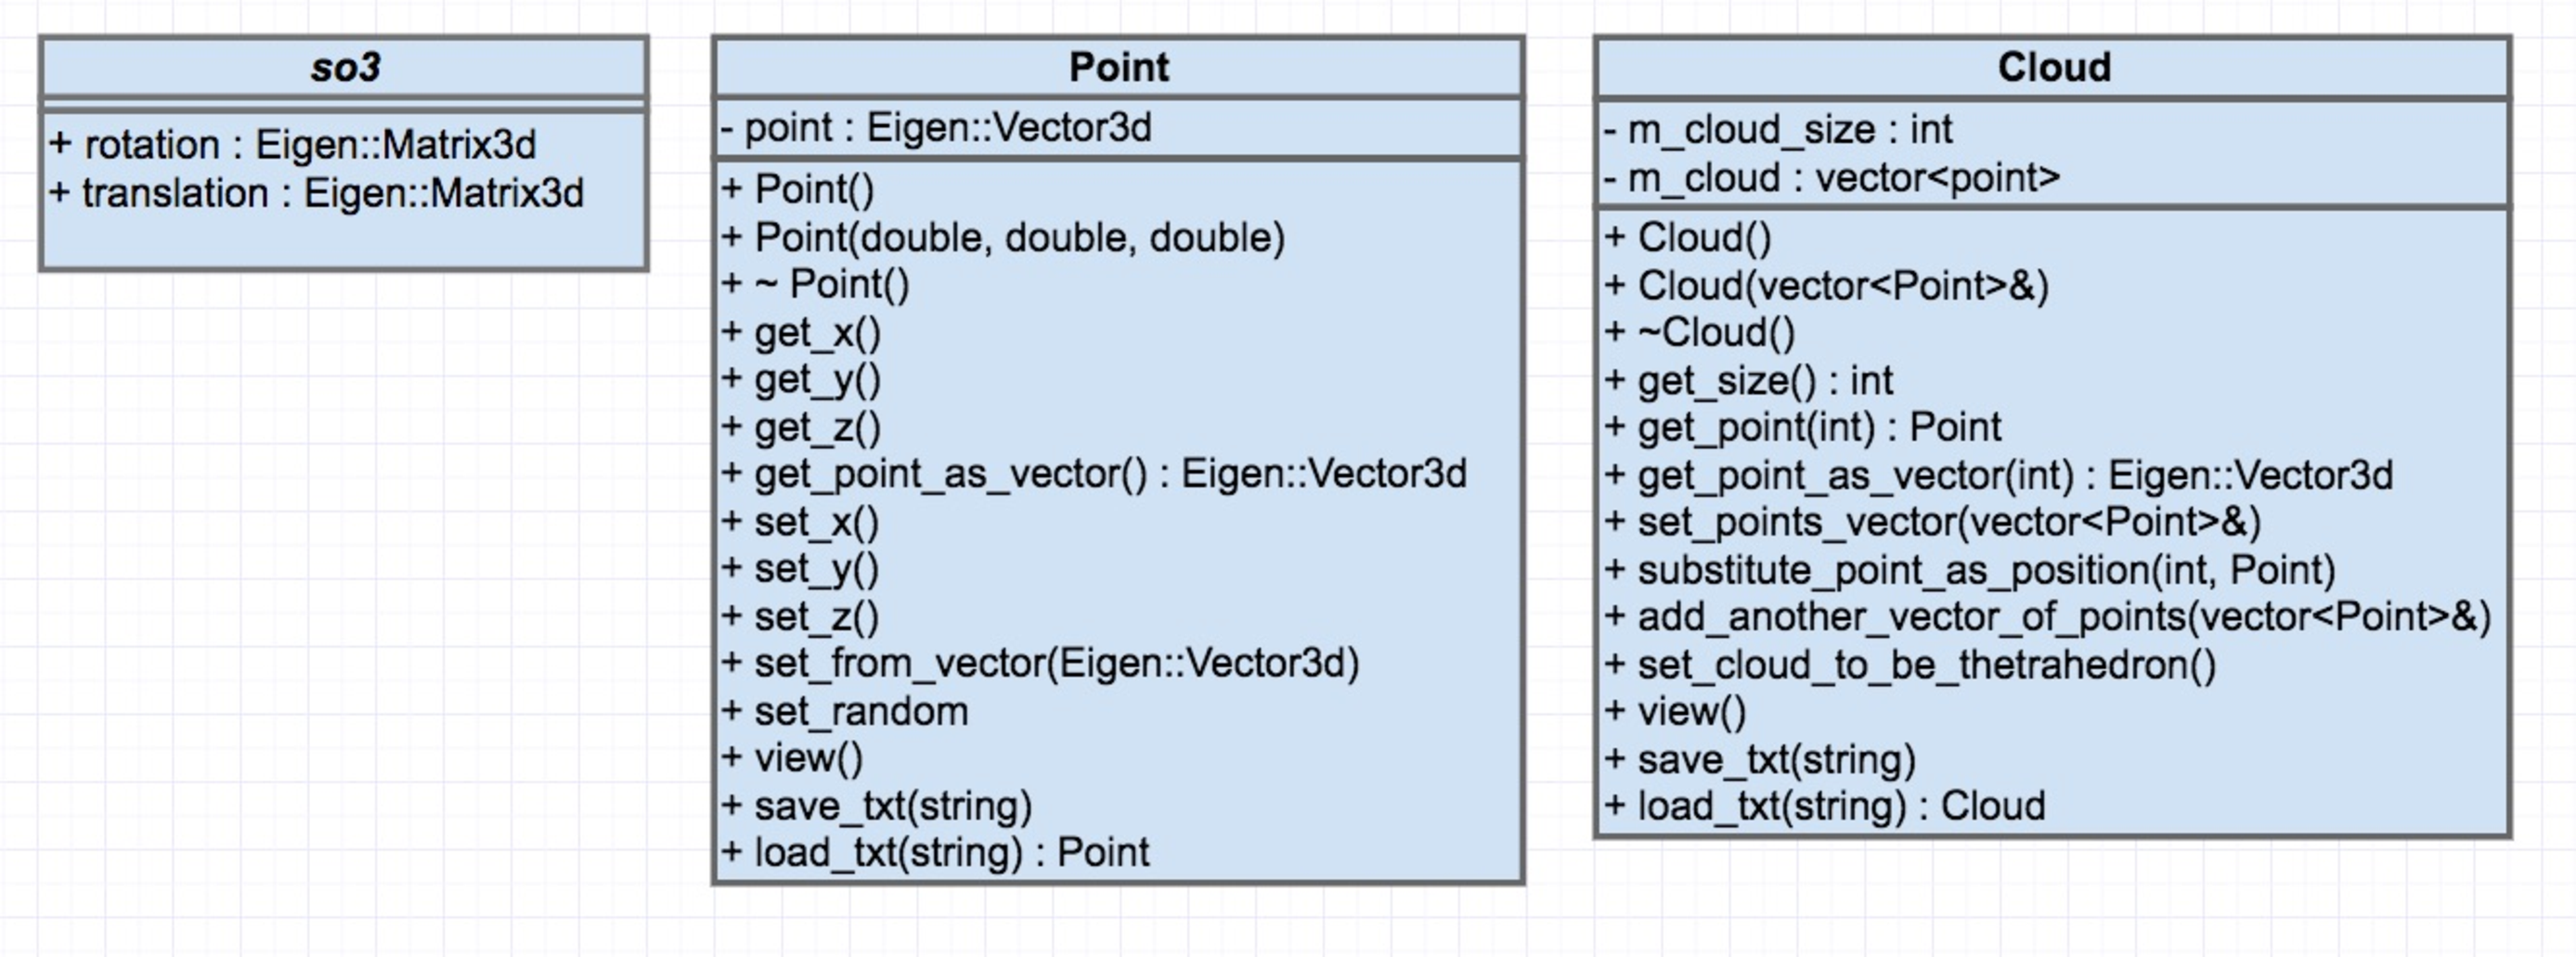
\includegraphics[scale=0.35]{figures/uml_diag.pdf}
%	\caption{UML diagram with the choice of the classes proposed for the implementation of the AHB algorithm.}
%	\label{fig:uml_diagram_classes}
%\end{figure}

\noindent
%\color{MidnightBlue} {\large  Exercise 2} \color{Black} \\
%\color{MidnightBlue}{\bf (a) }\color{Black} 
%Using the proposed framework, I implemented the AHB algorithm \cite{ahb_algo} in a simple folder structure under \emph{Code/registration\textunderscore3d\textunderscore point\textunderscore sets} divided into \emph{include}, \emph{source} and \emph{utils\textunderscore python}.
%\emph{Include} and \emph{source} contains respectively the header files and the source code. There are two .cc files with a main, that produces the actual applications: \emph{see\textunderscore methods.cc} and \emph{algo\textunderscore AHB.cc}. These can be called from the terminal under the path \emph{RCCPP-build/bin} in the build folder of the suggested framework. I choose an object oriented pattern, where one C++ structure, called \emph{so3}, and two classes, called \emph{Point} and \emph{Cloud}, are proposed. \\



\begin{center}
	\color{MidnightBlue} {\Large Part 2: Parallel computation - OpenMP }\color{Black} 
\end{center}


qsub command here!

\begin{center}
	\color{MidnightBlue} {\Large Part 2: Remote computation - OpenMP }\color{Black} 
\end{center}






\vspace{1cm}
\noindent
Please see the link include in the README.md on the github \href{https://github.com/SebastianoF/game_of_life}{repository} for references.
\end{document}





